\section{系统架构设计}

\subsection{系统架构图}
\begin{figure}[H]
\centering
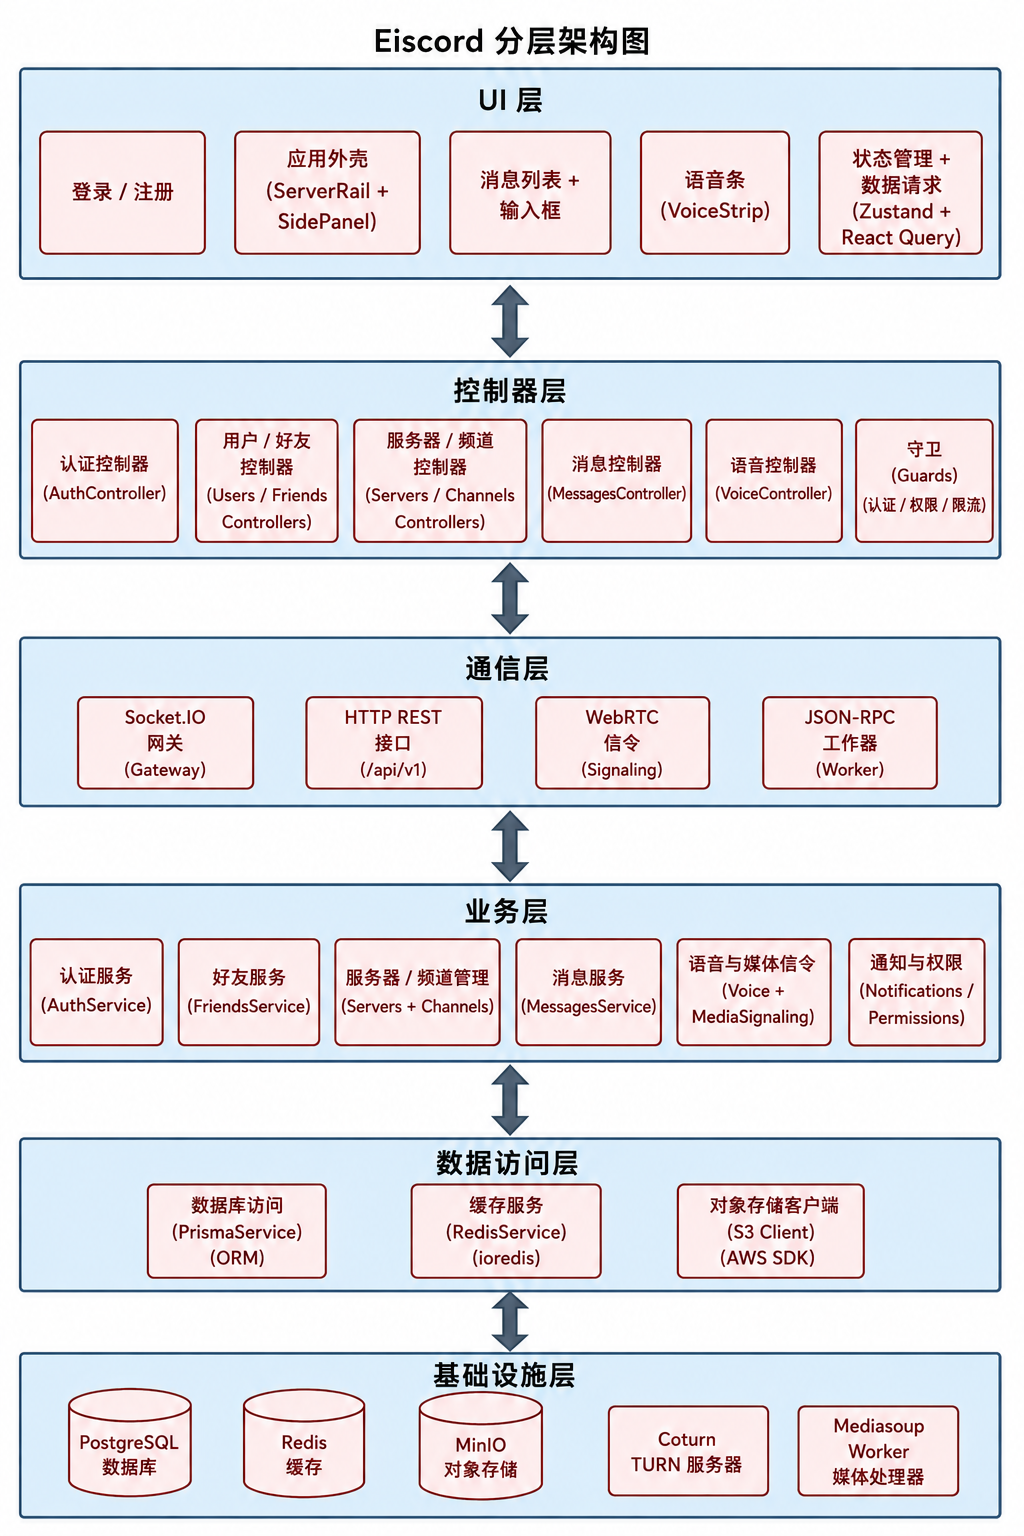
\includegraphics[width=\textwidth]{figures/arch-layers.png}
\caption{系统分层架构图}
\label{fig:architecture}
\end{figure}

\subsection{总体架构设计}
本系统采用前后端分离 + 三层架构设计：

\begin{description}[itemsep=0pt]
  \item[UI 层] React 18 SPA，Vite 构建，react-router-dom 路由，Zustand + React Query 状态管理，Socket.IO 客户端实时通信，mediasoup-client 语音媒体。
  \item[控制器层] NestJS Controllers + Guards（AccessToken / Permission / RateLimit）+ Filters / Interceptors。
  \item[通信层] HTTP REST（Axios）、WebSocket（Socket.IO 4.7）、WebRTC（mediasoup-client）、JSON-RPC（Worker 子进程）。
  \item[业务层] 14 个 NestJS Service 模块，覆盖认证、用户、好友、社区、频道、消息、语音、通知、权限等核心领域。
  \item[数据访问层] Prisma ORM（PostgreSQL）、ioredis（Redis）、AWS S3 SDK（MinIO）。
\end{description}

\subsection{核心模块划分}
\begin{center}
\captionof{table}{核心模块一览}
\begin{tabularx}{\textwidth}{L{2.8cm}L{2.5cm}Y}
\toprule
\textbf{模块} & \textbf{层级} & \textbf{职责} \\
\midrule
Auth 认证 & 业务层 & 注册/登录/JWT 签发/会话管理 \\
Users 用户 & 业务层 & 资料管理、在线状态 \\
Friends 好友 & 业务层 & 好友申请/关系维护/私聊会话 \\
Servers 社区 & 业务层 & 社区 CRUD/角色/成员/邀请 \\
Channels 频道 & 业务层 & 频道 CRUD/权限覆盖 \\
Messages 消息 & 业务层 & 消息发送/分页/已读/去重 \\
Voice 语音 & 业务层 & 语音频道加入/离开/状态同步 \\
MediaSignaling & 业务层 & WebRTC 信令/Mediasoup 编排 \\
Realtime 实时 & 业务+通信层 & Socket.IO 网关/事件广播/房间管理 \\
Notifications 通知 & 业务层 & 通知创建/列表/已读标记 \\
Attachments 附件 & 业务层 & S3 预签名上传/附件生命周期 \\
Permissions 权限 & 业务层 & bitmask 权限计算/校验 \\
Audit 审计 & 业务层 & 关键操作审计日志 \\
Health 健康 & 控制器层 & 服务健康检查 \\
\bottomrule
\end{tabularx}
\end{center}

\subsection{技术选型}
\begin{tabularx}{\textwidth}{L{3.5cm}L{3.5cm}L{4.5cm}}
\toprule
\textbf{层级} & \textbf{选型} & \textbf{版本} \\
\midrule
Web 客户端 & React + TypeScript + Vite & React 18.2 \\
服务端框架 & NestJS & 10.3.8 \\
ORM & Prisma & 5.13.0 \\
主数据库 & PostgreSQL（Docker） & 16 Alpine \\
缓存与状态 & Redis（Docker） & 7 Alpine \\
实时通信 & Socket.IO & 4.7.5 \\
语音媒体 & Mediasoup & 3.15.7 \\
对象存储 & MinIO / AWS S3 SDK & 3.1041.0 \\
TURN 中继 & Coturn & latest \\
数据验证 & Zod & 3.23.8 \\
状态管理 & Zustand + React Query & 4.5.2 / 5.32.1 \\
包管理 & pnpm monorepo & 9.15.4 \\
\bottomrule
\end{tabularx}

\subsection{模块间依赖关系}
\begin{itemize}[itemsep=0pt]
  \item Controller $\to$ Service $\to$ PrismaService（垂直调用）
  \item MessagesService 依赖 NotificationsService、RealtimePublisher
  \item VoiceService / MediaSignalingService 依赖 MediasoupWorkerClient、MediasoupRouterRegistry
  \item FriendsService 依赖 NotificationsService
  \item 权限校验链路：AccessTokenGuard $\to$ PermissionGuard $\to$ RateLimitGuard
  \item 请求链路：RequestIdMiddleware $\to$ ApiExceptionFilter $\to$ ApiResponseInterceptor
\end{itemize}
